\caulc

\Opensolutionfile{ans}[ans-ABCD]

%%%==============Cau_EX1==============%%%
\begin{ex}%%[1D1N1-3]%[CTST - Lớp 11 - Ôn tập giữa học kì 1 - Đề 3]%[Nguyễn Mộng Hùng]
	Cho góc lượng giác $(Ou,Ov)$ có số đo là $\dfrac{\pi}{3}$. Các góc lượng giác sau đây có cùng tia đầu $Ou$, hỏi góc nào có tia cuối $Ov$?
	\choice
	{$\dfrac{2\pi}{3}$}
	{$-\dfrac{2\pi}{3}$}
	{$\dfrac{5\pi}{3}$}
	{\True $-\dfrac{5\pi}{3}$}
	\loigiai{
		Hai góc có cùng tia đầu và tia cuối khi số đo của chúng chênh lệch nhau một bội số nguyên lần $2\pi$.\\
		Ta thấy
		$\dfrac{\pi}{3}-\left(-\dfrac{5\pi}{3}\right)=2\pi$.
	}
\end{ex}
%%%==============Cau_EX2==============%%%
\begin{ex}%%[1D1N1-3]%[CTST - Lớp 11 - Ôn tập giữa học kì 1 - Đề 3]%[Nguyễn Mộng Hùng]
	Cho góc lượng giác $(Ou,Ov)$ có số đo $\dfrac{3\pi}{4}$, góc lượng giác $(Ou,Ow)$ có số đo $\dfrac{5\pi}{4}$ Số đo của góc lượng giác $(Ov,Ow)$ là
	\choice
	{\True $\dfrac{\pi}{2}+k2\pi$}
	{$-\dfrac{\pi}{2}+k2\pi$}
	{$-\dfrac{\pi}{3}+k2\pi$}
	{$\dfrac{\pi}{3}+k2\pi$}
	\loigiai{
		Ta có $\text{sđ}(Ov,Ow)=\text{sđ}(Ou,Ow)-\text{sđ}(Ou,Ov)+k2\pi=\dfrac{5\pi}{4}-\dfrac{3\pi}{4}+k2\pi=\dfrac{\pi}{2}+k2\pi$.
	}
\end{ex}

%%%==============Cau_EX3==============%%%
\begin{ex}%%[1D1N4-4]%[CTST - Lớp 11 - Ôn tập giữa học kì 1 - Đề 3]%[Nguyễn Mộng Hùng]
	Khẳng định nào dưới đây là \textbf{sai}?
	\choice
	{\True Hàm số $y=\cos x$ là hàm số lẻ}
	{Hàm số $y=\cot x$ là hàm số lẻ}
	{Hàm số $y=\sin x$ là hàm số lẻ}
	{Hàm số $y=\tan x$ là hàm số lẻ}
	\loigiai{
		Ta có hàm số $y=\cos x$ là hàm số chẵn.
	}
\end{ex}


%%%==============Cau_EX4==============%%%
\begin{ex}%%[1D1N1-2]%[CTST - Lớp 11 - Ôn tập giữa học kì 1 - Đề 3]%[Nguyễn Mộng Hùng]
	Cung có số đo $250^\circ$ thì có số đo theo đơn vị là radian là
	\choice
	{$\dfrac{25\pi}{12}$}
	{\True $\dfrac{25\pi}{18}$}
	{$\dfrac{25\pi}{9}$}
	{$\dfrac{35\pi}{18}$}
	\loigiai{
		Ta có $250^\circ=\dfrac{250\pi}{180}=\dfrac{25\pi}{18}$.
	}
\end{ex}
%%%==============Cau_EX5==============%%%
\begin{ex}%%[1D1N4-2]%[CTST - Lớp 11 - Ôn tập giữa học kì 1 - Đề 3]%[Nguyễn Mộng Hùng]
	Tập xác định của hàm số $y=\dfrac{1}{\sin x}$ là
	\choice
	{$\mathscr{D}=\mathbb{R}\setminus\left\{\dfrac{\pi}{2}+k\pi|k\in\mathbb{Z}\right\}$}
	{$\mathscr{D}=\mathbb{R}\setminus\{k2\pi|k\in\mathbb{Z}\}$}
	{$\mathscr{D}=\mathbb{R}\setminus\left\{\dfrac{\pi}{2}+k2\pi|k\in\mathbb{Z}\right\}$}
	{\True $\mathscr{D}=\mathbb{R}\setminus\{k\pi|k\in\mathbb{Z}\}$}
	\loigiai{
		Điều kiện $\sin x\neq 0\Leftrightarrow x\neq k\pi,k\in\mathbb{Z}$.\\
		Tập xác định $\mathscr{D}=\mathbb{R}\setminus\{k\pi|k\in\mathbb{Z}\}$.
	}
\end{ex}


%%%==============Cau_EX6==============%%%
\begin{ex}%%[1D1N5-3]%[CTST - Lớp 11 - Ôn tập giữa học kì 1 - Đề 3]%[Nguyễn Mộng Hùng]
	Nghiệm của phương trình $\cos x=\dfrac{\sqrt{2}}{2}$ là
	\choice
	{$x=\dfrac{\pi}{2}+k2\pi,k\in\mathbb{Z}$ hoặc $x=\dfrac{\pi}{2}+k2\pi,k\in\mathbb{Z}$}
	{$x=\dfrac{\pi}{3}+k2\pi,k\in\mathbb{Z}$ hoặc $x=\dfrac{\pi}{3}+k2\pi,k\in\mathbb{Z}$}
	{\True $x=\dfrac{\pi}{4}+k2\pi, k\in\mathbb{Z}$ hoặc $x=-\dfrac{\pi}{4}+k2\pi,k\in\mathbb{Z}$}
	{$x=\dfrac{\pi}{6}+k2\pi, k\in\mathbb{Z}$ hoặc $x=-\dfrac{\pi}{6}+k2\pi,k\in\mathbb{Z}$}
	\loigiai{
		Ta có
		$\cos x=\dfrac{\sqrt{2}}{2}$
		$\Leftrightarrow\cos x=\cos\dfrac{\pi}{4}$
		$\Leftrightarrow\hoac{&x=\dfrac{\pi}{4}+k2\pi\\
			&x=-\dfrac{\pi}{4}+k2\pi
		}(k\in\mathbb{Z})$.
	}
\end{ex}

%%%==============Cau_EX7==============%%%
\begin{ex}%%[1D2H1-4]%[CTST - Lớp 11 - Ôn tập giữa học kì 1 - Đề 3]%[Nguyễn Mộng Hùng]
	Dãy số nào trong các dãy số dưới đây là dãy số giảm?
	\choice
	{$(u_n)$ với $u_n=3n$}
	{\True $(u_n)$ với $u_n=\dfrac{2}{n}$}
	{$(u_n)$ với $u_n=n^2$}
	{$(u_n)$ với $u_n=n+2$}
	\loigiai{
		\begin{itemize}
			\item Xét $(u_n)$ với $u_n=3n$\\
			Ta có $u_{n+1}=3(n+1)=3n+3> 3n=u_n,\forall n\in\mathbb{N}^*$. Vậy $(u_n)$ là dãy số tăng.
			\item Xét $(u_n)$ với $u_n=\dfrac{2}{n}$.\\
			Ta có $u_{n+1}=\dfrac{2}{n+1} < \dfrac{2}{n}=u_n,\forall n\in\mathbb{N}^*$. Vậy $(u_n)$ là dãy số giảm.
			\item Xét $(u_n)$ với $u_n=n^2$.\\
			Ta có $u_{n+1}=(n+1)^2> n^2=u_n,\forall n\in\mathbb{N}^*$. Vậy $(u_n)$ là dãy số tăng.
			\item Xét $(u_n)$ với $u_n=n+2$.\\
			Ta có $u_{n+1}=(n+1)+2=n+3> n+2=u_n,\forall n\in\mathbb{N}$. Vậy $(u_n)$ là dãy số tăng.
		\end{itemize}
		
		
	}
\end{ex}
%%%==============Cau_EX8==============%%%
\begin{ex}%[1D2N2-2]%[CTST - Lớp 11 - Ôn tập giữa học kì 1 - Đề 3]%[Nguyễn Mộng Hùng]
	Dãy số nào trong các dãy số dưới đây là một cấp số cộng?
	\choice
	{\True $1; 4; 7;10;13$}
	{$1;5;10;15; 20$}
	{$6;6;6;6;7$}
	{$3;6;9;12;13$}
	\loigiai{
		\begin{itemize}
			\item Dãy số  $1$; $4$; $7$; $10$; $13$  là một cấp số cộng với công sai $d=3$.
			\item Dãy số  $1$; $5$; $10$; $15$; $20$  có $u_2-u_1=4\neq u_3-u_2=5$ nên không phải là một cấp số.
			\item Dãy số  $6$; $6$; $6$; $6$; $7$  có $u_4-u_3=0\neq u_5-u_4=1$ nên không phải là một cấp số.
			\item Dãy số  $3$; $6$; $9$; $12$; $13$  có $u_4-u_3=3\neq u_5-u_4=1$ nên không phải là một cấp số.
		\end{itemize}
	
	}
\end{ex}

%%%==============Cau_EX9==============%%%
\begin{ex}%[1D2H2-6]%[CTST - Lớp 11 - Ôn tập giữa học kì 1 - Đề 3]%[Nguyễn Mộng Hùng]
	Cho cấp số cộng $(u_n)$ có $u_5=-15, u_{20}=60$. Tổng của 10 số hạng đầu tiên của cấp số cộng này là
	\choice
	{\True $S_{10}=-125$}
	{$S_{10}=-250$}
	{$S_{10}=200$}
	{$S_{10}=-200$}
	\loigiai{
		Gọi $u_1$, $d$ lần lượt là số hạng đầu và công sai của cấp số cộng.\\
		Ta có $\begin{cases}
			u_5=-15\\
			u_{20}=60\end{cases}$
		$\Leftrightarrow \begin{cases}
			u_1+4d=-15\\
			u_1+19d=60\end{cases}$
		$\Leftrightarrow \begin{cases}
			d=5\\
			u_1=-35.\end{cases}$\\
		Vậy $S_{10}=\dfrac{10}{2}(2u_1+9d)=5.[2.(-35)+9.5]=-125$.
	}
\end{ex}


%%%==============Cau_EX10==============%%%
\begin{ex}%[1D3H1-1]%[CTST - Lớp 11 - Ôn tập giữa học kì 1 - Đề 3]%[Nguyễn Mộng Hùng]
	Cho dãy số $(u_n)$ thoả $|u_n-3|< \dfrac{1}{n^5}$ với mọi $n\in\mathbb{N}^*$. Khẳng định nào sau đây \textbf{đúng}?
	\choice
	{$\lim\limits_{n\to+\infty}u_n=-3$}
	{$\lim\limits_{n\to+\infty}u_n=5$}
	{$\lim\limits_{n\to+\infty}u_n=0$}
	{\True $\lim\limits_{n\to+\infty}u_n=3$}
	\loigiai{
		Ta có $|u_n-3|< \dfrac{1}{n^5}$ với mọi $n\in\mathbb{N}^*$. Mà $\lim\limits_{n\to\infty}\dfrac{1}{n^5}=0$\\
		Suy ra $\lim\limits_{n\to+\infty}(u_n-3)=0$
		$\Rightarrow\lim\limits_{n\to+\infty}u_n=3$.
	}
\end{ex}


%%%==============Cau_EX11==============%%%
\begin{ex}%[1D3H2-3]%[CTST - Lớp 11 - Ôn tập giữa học kì 1 - Đề 3]%[Nguyễn Mộng Hùng]
	$\lim\limits_{x\to-1}\dfrac{x^2-2x-3}{x+1}$ bằng
	\choice
	{$0$}
	{\True $-4$}
	{$-3$}
	{$1$}
	\loigiai{
		Ta có $\lim\limits_{x\to-1}\dfrac{x^2-2x-3}{x+1}=\lim\limits_{x\to-1}\dfrac{(x+1)(x-3)}{x+1}=\lim\limits_{x\to-1}(x-3)=-4$.
	}
\end{ex}


%%%==============Cau_EX12==============%%%
\begin{ex}%[1D3H3-3]%[CTST - Lớp 11 - Ôn tập giữa học kì 1 - Đề 3]%[Nguyễn Mộng Hùng]
	Cho hàm số $f(x)=\heva{&\dfrac{\sqrt{x+2}-2}{x-2}&\text{khi}\, x\neq 2\\&4& \text{khi}\, x=2}$. Chọn mệnh đề \textbf{đúng}.
	\choice
	{Hàm số liên tục tại $x=2$}
	{\True Hàm số gián đoạn tại $x=2$}
	{$f(4)=2$}
	{$\lim\limits_{x\to 2}f(x)=2$}
	\loigiai{
		Tập xác định: $\mathscr{D}=\mathbb{R}$.\\
		\begin{eqnarray*}
			\lim\limits_{x\to 2}f(x)&=&\lim\limits_{x\to 2}\dfrac{\sqrt{x+2}-2}{x-2}\\
			&=&\lim\limits_{x\to 2}\dfrac{(\sqrt{x+2}-2)(\sqrt{x+2}+2)}{(x-2)(\sqrt{x+2}+2)}\\
			&=&\lim\limits_{x\to 2}\dfrac{x-2}{(x-2)(\sqrt{x+2}+2)}\\
			&=&\lim\limits_{x\to 2}\dfrac{1}{\sqrt{x+2}+2}=\dfrac{1}{4}.
		\end{eqnarray*}
		Mà $f(2)=4$. Do đó $\lim\limits_{x\to 2}f(x)\neq f(2)$.\\
		  Vậy hàm số gián đoạn tại $x=2$. 
	}
\end{ex}

\Closesolutionfile{ans}

\indapan{6}{ans-ABCD}

\cauds

\Opensolutionfile{ans}[ans-DS]
%%%%==============Cau_EX1==============%%%
\begin{ex}%[1D1H4-4]%[CTST - Lớp 11 - Ôn tập giữa học kì 1 - Đề 3]%[Nguyễn Mộng Hùng]
	Cho hàm số $f(x)=\sin\left(\dfrac{\pi}{2}-2x\right)+2024$.
	\choiceTF
	{\True Hàm số $f(x)$ có tập xác định là $\mathbb{R}$}
	{\True Chu kỳ của hàm số $f(x)$ là $T=2\pi$}
	{Hàm số $f(x)$ không chẵn, không lẻ}
	{\True Hàm số $f(x)$ nghịch biến trên khoảng $\left(k\pi;\dfrac{\pi}{2}+k\pi\right)$ với $k\in\mathbb{Z}$}
	\loigiai{
		\begin{itemchoice}
			\itemch Đúng. Hàm số $f(x)=\sin\left(\dfrac{\pi}{2}-2x\right)+2024$ luôn xác định $\forall x\in\mathbb{R}$.\\
			 Nên hàm số $f(x)$ có tập xác định là $\mathbb{R}$
			\itemch Đúng. Ta có $f(x)=\sin\left(\dfrac{\pi}{2}-2x\right)+2024=\cos 2x+2024$.\\
			 Nên hàm số $f(x)$ tuần hoàn với chu ki $T=\dfrac{2\pi}{2}=\pi$.
			\itemch Sai. Ta có $\forall x\in\mathbb{R},-x\in\mathbb{R}$.\\
			 Và $f(-x)=\cos(-2x)+2024=\cos 2x+2024=f(x)$.\\
			  Nên hàm số $f(x)$ là hàm số chẵn.
			\itemch Đúng. Hàm số $y=\cos 2x+2024$ nghịch biến khi\\ $k2\pi < 2x < \pi+k2\pi\Leftrightarrow k\pi < x < \dfrac{\pi}{2}+k\pi,k\in\mathbb{Z}$.\\
			Do đó hàm số $f(x)$ nghịch biến trên khoảng $\left(k\pi;\dfrac{\pi}{2}+k\pi\right)$ với $k\in\mathbb{Z}$.
		\end{itemchoice}
	}
\end{ex}


%%%==============Cau_EX2==============%%%
\begin{ex}%[1D1V5-3]%[CTST - Lớp 11 - Ôn tập giữa học kì 1 - Đề 3]%[Nguyễn Mộng Hùng]
	Phương trình $\sin 3x=\sin x$.
	\choiceTF
	{\True Tập nghiệm của phương trình là $S=\left\{ k\pi;\dfrac{\pi}{4}+\dfrac{k\pi}{2}\vert k\in\mathbb{Z}\right\}$}
	{\True Nghiệm dương nhỏ nhất của phương trình là $x=\dfrac{\pi}{4}$}
	{Phương trình đã cho tương đương với phương trình $\sin 2x-1=0$}
	{\True Tổng các nghiệm thuộc đoạn $\left[-\pi;\dfrac{5\pi}{2}\right]$ của phương trình bằng $\dfrac{29\pi}{4}$}
	\loigiai{
		\begin{itemchoice}
			\itemch Đúng.
			Ta có $\sin 3x=\sin x\Leftrightarrow\hoac{&3x=x+k2\pi\\
				&3x=\pi-x+k2\pi}\Leftrightarrow\hoac{&x=k\pi\\
				&x=\dfrac{\pi}{4}+\dfrac{k\pi}{2}}$ $(k\in\mathbb{Z})$.\\
			Nên $S=\left\{k\pi;\dfrac{\pi}{4}+\dfrac{k\pi}{2},k\in\mathbb{Z}\right \}$.
			\itemch Đúng.
			Với $x=k\pi(k\in\mathbb{Z})$ thì nghiệm dương nhỏ nhất là $\pi$.\\
			Với $x=\dfrac{\pi}{4}+\dfrac{k\pi}{2}(k\in\mathbb{Z})$ thì nghiệm dương nhỏ nhất là $\dfrac{\pi}{4}$.\\
			Vậy nghiệm dương nhỏ nhất của phương trình là $x=\dfrac{\pi}{4}$.
			\itemch Sai.
			Ta có $\sin 2x-1=0\Leftrightarrow 2x=\dfrac{\pi}{2}+k2\pi\Leftrightarrow x=\dfrac{\pi}{4}+k\pi\,(k\in\mathbb{Z})$.\\
			Nên $S_1=\left\{\dfrac{\pi}{4}+k\pi, k\in\mathbb{Z}\right\}$.\\
			Do $S_1\neq S$ nên phương trình đã cho không tương đương với phương trình\\
			 $\sin 2x-1=0$.
			\itemch  Đúng.
			\begin{itemize}
				\item Với $x=k\pi(k\in\mathbb{Z})$, các nghiệm thuộc đoạn $\left[-\pi;\dfrac{5\pi}{2}\right]$ là $x\in\{-\pi;0;\pi;2\pi\}$.
				\item Với $x=\dfrac{\pi}{4}+\dfrac{k\pi}{2}(k\in\mathbb{Z})$, các nghiệm thuộc đoạn $\left[-\pi;\dfrac{5\pi}{2}\right]$ là\\ $x\in\left\{\dfrac{-3\pi}{4};\dfrac{-\pi}{4};\dfrac{\pi}{4};\dfrac{3\pi}{4};\dfrac{5\pi}{4};\dfrac{7\pi}{4};\dfrac{9\pi}{4}\right\}$.
				\item Tổng các nghiệm thuộc đoạn $\left[-\pi;\dfrac{5\pi}{2}\right]$ của phương trình là\\
				$-\pi+0+\pi+2\pi+\dfrac{-3\pi}{4}+\dfrac{-\pi}{4}+\dfrac{\pi}{4}+\dfrac{3\pi}{4}+\dfrac{5\pi}{4}+\dfrac{7\pi}{4}+\dfrac{9\pi}{4}=\dfrac{29\pi}{4}$.
			\end{itemize}
			
		\end{itemchoice}
	}
\end{ex}


%%%==============Cau_EX3==============%%%
\begin{ex}%[1D2V2-6]%[CTST - Lớp 11 - Ôn tập giữa học kì 1 - Đề 3]%[Nguyễn Mộng Hùng]
	Cho cấp số cộng $(u_n)$ biết $\heva{&u_1=2\\&u_{n+1}=u_n+5}$ với $n\geq 1, n\in\mathbb{N}$.
	\choiceTF
	{\True Số hạng thứ hai của cấp số cộng là $u_2=7$}
	{\True Công sai của cấp số cộng $d=5$}
	{Số hạng tổng quát của cấp số cộng đã cho $u_n=5n+3$}
	{\True Tổng các số hạng từ số hạng thứ $11$ đến số hạng thứ 100 của cấp số cộng đã cho bằng $25\,705$}
	\loigiai{
		\begin{itemchoice}
			\itemch Đúng.
			$u_2=u_1+5=2+5=7$.
			\itemch Đúng.
			$u_{n+1}=u_n+5\Leftrightarrow u_{n+1}-u_n=5\Leftrightarrow d=5$, với $\forall n\in\mathbb{N}^*$.
			\itemch Sai.
			$u_n=u_1+(n-1)d=2+(n-1).5=5n-3$, với $\forall n\in\mathbb{N}^*$.
			\itemch Đúng.
			$S_{10}=\dfrac{10\cdot(u_1+u_{10})}{2}=\dfrac{10\cdot(2+47)}{2}=245$.\\
			$S_{100}=\dfrac{100.(u_1+u_{100})}{2}=\dfrac{100\cdot(2+497)}{2}=25\,950$.\\
			Vậy $S=u_{11}+u_{21}+\cdots+u_{100}=S_{100}-S_{10}=25\,705$.
		\end{itemchoice}
	}
\end{ex}


%%%==============Cau_EX4==============%%%
\begin{ex}%[1D3V3-3]%[CTST - Lớp 11 - Ôn tập giữa học kì 1 - Đề 3]%[Nguyễn Mộng Hùng]
	Cho hàm số $f(x)=\heva{&\dfrac{2x^2+3x-5}{x-1}&\text{khi}\,x < 1\\
		&24x-8&\text{khi}\,x\geq 1.}$
	\choiceTF
	{\True $f(1)=16$}
	{$\lim\limits_{x\to 1}f(x)=16$}
	{Hàm số liên tục tại $x=1$}
	{\True $\lim\limits_{x\to 1^-}\dfrac{f(x)-16}{(x-1)(\sqrt{2f(x)+4}+6)}=2$}
	\loigiai{
	\begin{itemchoice}
		\itemch Đúng.
		Với $x=1$ thì $f(x)=24x-8$ suy ra $f(1)=24\cdot 1-8=16$.
		\itemch Sai.
		$\lim\limits_{x\to 1^-}f(x)=\lim\limits_{x\to 1^-}\dfrac{2x^2+3x-5}{x-1}=\lim\limits_{x\to 1^-}\dfrac{(x-1)(2x+5)}{x-1}=\lim\limits_{x\to 1^-}(2x+5)=7$.
		\itemch Sai.
		$\lim\limits_{x\to 1^-}f(x)\neq\lim\limits_{x\to 1^+}f(x)=f(1)$.
		\itemch Đúng.
		
		\begin{eqnarray*}
			&&\lim\limits_{x\to 1^-}\dfrac{f(x)-16}{(x-1)\left(\sqrt{2f(x)+4}+6\right)}\\
			&=&\lim\limits_{x\to 1^-}\dfrac{24(x-1)}{(x-1)\left(\sqrt{2f(x)+4}+6\right)}\\
			&=&24\cdot\dfrac{1}{\sqrt{2f(1)+4}+6}=2
		\end{eqnarray*}
	\end{itemchoice}
	}
\end{ex}

\Closesolutionfile{ans}

\indapan{3}{ans-DS}

\caukq

\Opensolutionfile{ans}[ans-KQ]

%%%==============Bai_BT1==============%%%
\begin{ex}%[1D1V5-3]%[CTST - Lớp 11 - Ôn tập giữa học kì 1 - Đề 3]%[Nguyễn Mộng Hùng]
	Phương trình $\sin\left(3x+\dfrac{\pi}{3}\right)=-\dfrac{\sqrt{3}}{2}$ có $\overline{abcd}$ (số có bốn chữ số) nghiệm thuộc khoảng $(-2024;2025)$. Tính $a+b+c+d$.
	\shortans{$24$}
	\loigiai{
		Ta có
		\begin{eqnarray*}
			&&\sin\left(3x+\dfrac{\pi}{3}\right)=-\dfrac{\sqrt{3}}{2}\\
			&\Leftrightarrow&\hoac{&3x+\dfrac{\pi}{3}=-\dfrac{\pi}{3}+k2\pi\\&3x+\dfrac{\pi}{3}=\dfrac{4\pi}{3}+l2\pi}\\
			 &\Leftrightarrow& \hoac{&3x=-\dfrac{2\pi}{3}+k2\pi \\&3x=\pi+l2\pi}\\
			 &\Leftrightarrow& \hoac{&x=-\dfrac{2\pi}{9}+k\dfrac{2\pi}{3} \\&x=\dfrac{\pi}{3}+l\dfrac{2\pi}{3}}\,(k,l\in \mathbb{Z}).
		\end{eqnarray*}
		Vì $x\in(-2024;2025)$ nên\\
		$\hoac{&-2024<-\dfrac{2\pi}{9}+k\dfrac{2\pi}{3} < 2025\\&-2024< \dfrac{\pi}{3}+l\dfrac{2\pi}{3} < 2025}$
		$\Leftrightarrow \hoac{&-\dfrac{2024\cdot 9}{6\pi} < k < \dfrac{2025\cdot 9}{6\pi} \\&-\dfrac{2024\cdot3}{2\pi} < l < \dfrac{2025\cdot3}{2\pi}}\Leftrightarrow \hoac{&k=-966;\ldots; 966\\&l=-966;\ldots; 965.}$\\
		Do đó phương trình đã cho có $3\,867$ nghiệm thuộc khoảng $(-2024;2025)$.\\
		Vậy $a+b+c+d=3+8+6+7=24$.
	}
\end{ex}


%%%==============Bai_BT2==============%%%
\begin{ex}%[1D1V5-6]%[CTST - Lớp 11 - Ôn tập giữa học kì 1 - Đề 3]%[Nguyễn Mộng Hùng]
	Số giờ có ánh sáng của một thành phố trong ngày thứ $t$ của một năm không nhuận được cho bởi hàm số: $s(t)=3\sin\left[\dfrac{\pi}{182}(t-80)\right]+12$, $t\in\mathbb{Z}$ và $0< t\le 365$. Vào ngày thứ mấy trong năm thì thành phố đó có nhiều giờ ánh sáng nhất?
	\shortans{$171$}
	\loigiai{
		Ta có $s(t)=3\sin\left[\dfrac{\pi}{182}(t-80)\right]+12\le 3+12=15$.\\
		Dấu bằng xảy ra khi\\ $\sin\left[\dfrac{\pi}{182}(t-80)\right]=1\Leftrightarrow\dfrac{\pi}{182}(t-80)=\dfrac{\pi}{2}+k2\pi(k\in\mathbb{Z})\Leftrightarrow t=171+364k$.\\
		Mặt khác $t\in(0;365]$ nên $0< 171+364k\le 365\Leftrightarrow-\dfrac{171}{364} < k\le\dfrac{194}{364}$.\\
		 Mà $k\in\mathbb{Z}$ nên $k=0$. Do đó $t=171$.\\
		 Vậy ngày thứ $171$ trong năm thì thành phố đó có nhiều giờ ánh sáng nhất.
	}
\end{ex}
%%%==============Bai_BT3==============%%%
\begin{ex}%[1D2V2-7]%[CTST - Lớp 11 - Ôn tập giữa học kì 1 - Đề 3]%[Nguyễn Mộng Hùng]
	Công ty $A$ muốn thuê một mảnh đất trong vòng $15$ năm để làm nhà kho. Có hai công ty môi giới bất động sản $B$ và bất động sản $C$ đều muốn cho thuê. Mỗi công ty, đưa ra phương án cho thuê như sau:\\
	Phương án công ty $B$ trả tiền theo quý, quý đầu tiên là $10$ triệu đồng và từ quý thứ hai trở đi mỗi quý tăng thêm $500\,000$ đồng.\\
	Phương án công ty $C$ trả tiền theo năm, năm đầu tiên thuê đất là $70$ triệu và kể từ năm thứ hai trở đi mỗi năm tăng thêm $3$ triệu đồng.\\
	Nếu công ty $A$ lựa chọn thuê đất của công ty môi giới bất động sản nào để chi phí là thấp nhất và số tiền đó bằng $\overline{abcd}$ triệu đồng. Hỏi $a+b+c+d$ bằng bao nhiêu?
	\shortans{$15$}
	\loigiai{
		Gọi $B_n$, $C_n$ lần lượt là số tiền công ty $A$ cần trả theo cách tính của hai công ty $B$ và $C$
		Theo bài ra, ta có
		\begin{itemize}
			\item $B_n$ là tổng $n$ số hạng đầu tiên của một cấp số cộng với $u_1=10$ triệu đồng và công sai $d=0,5$ triệu đồng.
			\item $C_n$ là tổng $n$ số hạng đầu tiên của một cấp số cộng với $u_1=70$ triệu đồng, công sai $d=3$ triệu đồng.
		\end{itemize}
		Khi đó:\\
		Nếu thuê đất của công ty $B$ trong vòng 15 năm thì số tiền công ty $A$ phải trả là
		$$B_{60}=\dfrac{n}{2}\cdot[2u_1+(n-1)d]=30\cdot(2\cdot 10+59\cdot 0{,}5)=1\,485\, (\text{triệu đồng}).$$
		Nếu thuê đất của công ty $C$ trong vòng 15 năm thì số tiền công ty $A$ phải trả là
		$$C_{15}=\dfrac{n}{2}\cdot[2u_1+(n-1)d]=7{,}5(2\cdot70+14\cdot 3)=1\,365\, (\text{triệu đồng}).$$
		Do đó công ty $A$ nên thuê đất của công ty $C$ và số tiền phải trả là $1\,365$ (triệu đồng).\\
		Vậy $a+b+c+d=15$.
	}
\end{ex}
%%%==============Bai_BT4==============%%%
\begin{ex}%[1D2V3-8]%[CTST - Lớp 11 - Ôn tập giữa học kì 1 - Đề 3]%[Nguyễn Mộng Hùng]
	Trên một bàn cờ vua như hình. Các quân cờ Tốt, Mã, Tịnh, Xe, Hậu được tính điểm lần lượt là $1$, $3$, $3$, $5$, $9$. Giả sử quân Tốt trắng đang ở vị trí $E5$ và muốn được phong cấp Hậu ở vị trí $H8$ thì Tốt trắng sẽ ăn các quân cờ có điểm theo thứ tự lập thành một cấp số nhân. Tổng tất cả các số điểm của quân Tốt trắng ăn được bằng bao nhiêu?
	\begin{center}
		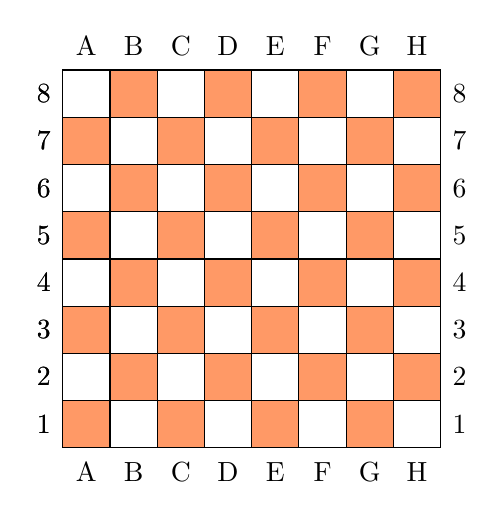
\begin{tikzpicture}[x=6mm,y=6mm]
			\definecolor{atomictangerine}{rgb}{1.0, 0.6, 0.4}
			\draw[fill=atomictangerine,even odd rule] (0,0) 
			foreach \n in {1,2,3,4} { -- ++ (8,0) -- ++ (0,1) -- ++ (-8,0) -- ++ (0,1) } -- (8,8)
			foreach \n in {1,2,3,4} { -- ++ (0,-8) -- ++ (-1,0) -- ++ (0,8) -- ++ (-1,0) } -- cycle
			foreach[count=\n] \m in {A,B,...,H} {(-0.4,\n-0.5) node {\n} (8.4,\n-0.5) node {\n} (\n-0.5,-0.5) node {\m}}
			foreach[count=\n] \m in {A,B,...,H} {(-0.4,\n-0.5) node {\n} (\n-0.5,8.5) node {\m}}
			;
		\end{tikzpicture}
	\end{center}
	\shortans{$13$}
	\loigiai{
		\begin{center}
			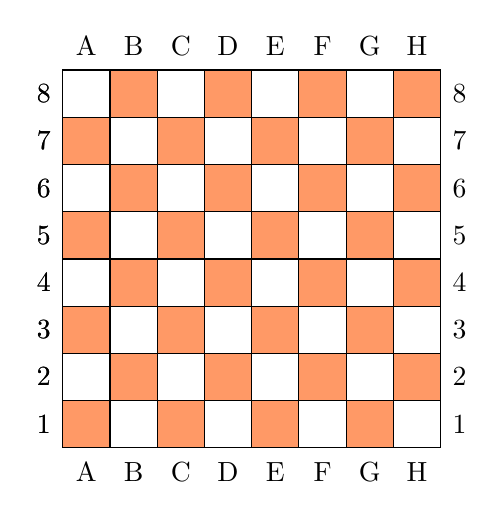
\begin{tikzpicture}[x=6mm,y=6mm]
				\definecolor{atomictangerine}{rgb}{1.0, 0.6, 0.4}
				\draw[fill=atomictangerine,even odd rule] (0,0) 
				foreach \n in {1,2,3,4} { -- ++ (8,0) -- ++ (0,1) -- ++ (-8,0) -- ++ (0,1) } -- (8,8)
				foreach \n in {1,2,3,4} { -- ++ (0,-8) -- ++ (-1,0) -- ++ (0,8) -- ++ (-1,0) } -- cycle
				foreach[count=\n] \m in {A,B,...,H} {(-0.4,\n-0.5) node {\n} (8.4,\n-0.5) node {\n} (\n-0.5,-0.5) node {\m}}
				foreach[count=\n] \m in {A,B,...,H} {(-0.4,\n-0.5) node {\n} (\n-0.5,8.5) node {\m}}
				;
			\end{tikzpicture}
		\end{center}
		Quân Tốt trắng đang ở vị trí $E5$ và muốn được phong cấp Hậu ở vị trí $H8$ thì Tốt trắng buộc ăn quân đen theo sơ đồ $F6\to G7\to H8$.
		\begin{itemize}
			\item Ở vị trí $H8$ có thể là các quân đen: Mã, Tịnh, Xe hoặc Hậu.
			\item Các số điểm mà quân Tốt trắng ăn được theo thứ tự lập thành $1$ cấp số nhân $1$, $3$, $9$ là $3$ số hạng cần tìm.
		\end{itemize}
		 Vậy tổng số điểm mà quân Tốt trắng ăn được là $1+3+9=13$.
	}
\end{ex}
%%%==============Bai_BT5==============%%%
\begin{ex}%[1D2V3-8]%[1D3V2-8]%[CTST - Lớp 11 - Ôn tập giữa học kì 1 - Đề 3]%[Nguyễn Mộng Hùng]
	Cho tam giác $OA_1A_2$ vuông tại $A_2$, $A_1A_2=2$ và $\widehat{A_1OA_2}=45^{\circ}$. Lần lượt hạ các đường vuông góc $A_2A_3\perp OA_1$; $A_3A_4\perp OA_2$; $A_4A_5\perp OA_1$; $A_5A_6\perp OA_2$; $\ldots$. Tiếp tục quá trình này, ta nhận được đường gấp khúc $A_1A_2A_3A_4\ldots$. Tính độ dài đường gấp khúc này (Làm tròn đến hàng phần trăm).
	\begin{center}
		\begin{tikzpicture}[declare function={r= 1.3;}]
			\path
			(0,0) coordinate (O)
			(r,0) coordinate (A_6)
			(2*r,0) coordinate (A_4)
			(4*r,0) coordinate (A_2)
			(4*r,4*r) coordinate (A_1)
			($(O)!.5!(A_1)$) coordinate (A_3)
			($(O)!.5!(A_3)$) coordinate (A_5)
			($(O)!.5!(A_5)$) coordinate (A_7)
			;
			\draw (O)--(A_2)--(A_1)--cycle (A_2)--(A_3)--(A_4)--(A_5)--(A_6)--(A_7)
			pic[draw,angle radius=5pt]{right angle= A_2--A_3--A_1}
			pic[draw,angle radius=5pt]{right angle= A_4--A_5--A_3}
			pic[draw,angle radius=5pt]{right angle= A_6--A_7--A_5}
			pic[draw,angle radius=5pt]{right angle= A_3--A_4--A_6}
			pic[draw,angle radius=5pt]{right angle= A_5--A_6--O}
			pic[draw,angle radius=5pt]{right angle= A_1--A_2--O}
			(O)pic[draw,angle radius = 15] {angle = A_2--O--A_1} node[shift={(22:22pt)},scale=.6]{$ 45^\circ $}	
			;
			
			\foreach \t/\g in {O/-90,A_6/-90,A_4/-90,A_2/-90,A_1/90,A_3/110,A_5/110,A_7/110}{
				\draw[fill=white] (\t) circle (1pt) node[shift={(\g:7pt)},font=\scriptsize]{$ \t $};
			}
		\end{tikzpicture}
	\end{center}
	\shortans{$4{,}83$}
	\loigiai{
		\begin{center}
			\begin{tikzpicture}[declare function={r= 1.3;}]
				\path
				(0,0) coordinate (O)
				(r,0) coordinate (A_6)
				(2*r,0) coordinate (A_4)
				(4*r,0) coordinate (A_2)
				(4*r,4*r) coordinate (A_1)
				($(O)!.5!(A_1)$) coordinate (A_3)
				($(O)!.5!(A_3)$) coordinate (A_5)
				($(O)!.5!(A_5)$) coordinate (A_7)
				;
				\draw (O)--(A_2)--(A_1)--cycle (A_2)--(A_3)--(A_4)--(A_5)--(A_6)--(A_7)
				pic[draw,angle radius=5pt]{right angle= A_2--A_3--A_1}
				pic[draw,angle radius=5pt]{right angle= A_4--A_5--A_3}
				pic[draw,angle radius=5pt]{right angle= A_6--A_7--A_5}
				pic[draw,angle radius=5pt]{right angle= A_3--A_4--A_6}
				pic[draw,angle radius=5pt]{right angle= A_5--A_6--O}
				pic[draw,angle radius=5pt]{right angle= A_1--A_2--O}
				(O)pic[draw,angle radius = 15] {angle = A_2--O--A_1} node[shift={(22:22pt)},scale=.6]{$ 45^\circ $}	
				;
				
				\foreach \t/\g in {O/-90,A_6/-90,A_4/-90,A_2/-90,A_1/90,A_3/110,A_5/110,A_7/110}{
					\draw[fill=white] (\t) circle (1pt) node[shift={(\g:7pt)},font=\scriptsize]{$ \t $};
				}
			\end{tikzpicture}
		\end{center}
		Các góc $\widehat{A_1A_2A_3}, \widehat{A_2A_3A_4}, \widehat{A_3A_4A_5}, \ldots$ đều bằng góc $\widehat{A_1OA_2}$ nên đều có đo là $45^{\circ}$.
		$$
		\begin{aligned}
			& A_2 A_3=A_1 A_2 \cdot \cos 45^{\circ}=2 \cdot \dfrac{\sqrt{2}}{2}=\sqrt{2}\\
			& A_3 A_4=A_2 A_3 \cdot \cos 45^{\circ}=2 \cdot \dfrac{\sqrt{2}}{2} \cdot \dfrac{\sqrt{2}}{2}=2\cdot\left(\dfrac{\sqrt{2}}{2}\right)^2 \\
			& A_4 A_5=A_3 A_4 \cdot \cos 45^{\circ}=2 \cdot\left(\dfrac{\sqrt{2}}{2}\right)^2 \cdot \dfrac{\sqrt{2}}{2}=2 \cdot\left(\dfrac{\sqrt{2}}{2}\right)^3; \ldots
		\end{aligned}
		$$
		Do đó độ dài các đoạn thẳng $A_1A_2$, $A_2A_3$, $A_3A_4$, $\ldots$ tạo thành cấp số nhân lùi vô hạn với số hạng đầu bằng $2$ với công bội bằng $\dfrac{\sqrt{2}}{2}$.\\
		Vậy độ dài đường gấp khúc $A_1A_2A_3A_4\ldots$ là $l=\dfrac{2}{1-\tfrac{\sqrt{2}}{2}}=2\sqrt{2}\cdot(\sqrt{2}+1)\approx 6{,}83$.
	}
\end{ex}
%%%==============Bai_BT6==============%%%
\begin{ex}%[1D3V2-8]%[CTST - Lớp 11 - Ôn tập giữa học kì 1 - Đề 3]%[Nguyễn Mộng Hùng]
	Trong hồ có chứa $2\,000$ lít nước ngọt. Người ta bơm nước biển có nồng độ muối là $40{,}5$ gam/lít vào hồ với tốc độ là $15$ lít/phút. Hỏi nồng độ muối trong hồ sau khi bơm thời gian $t$ phút là bao nhiêu nếu $t \to+\infty$?
	\shortans{$40{,}5$}
	\loigiai{
		Lượng nước biển mà người ta bơm vào trong khoảng thời gian t phút là $15t$.\\
		Lúc này lượng muối bơm vào là $40{,}5\cdot15t=607{,}5$.\\
		Nồng độ muối trong hồ lúc này là $\dfrac{607{,}5t}{2000+15t}$.\\
		Khi $t \to+\infty$, nồng độ muối trong hồ lúc này là
		$$
		\lim\limits_{x \to+\infty} \dfrac{607{,}5 t}{2\,000+15t}=\lim\limits_{x \to+\infty} \dfrac{607{,}5}{\frac{2\,000}{t}+15}=40{,}5.
		$$
	}
\end{ex}


\Closesolutionfile{ans}

\indapan{6}{ans-KQ}